% Chapter Template

\chapter{Ensayos y resultados} % Main chapter title

\label{Chapter4} % Change X to a consecutive number; for referencing this chapter elsewhere, use \ref{ChapterX}

En este capítulo se describen los ensayos que se realizaron y las métricas obtenidas. Además, se detallan los errores más comunes encontrados y ejemplos de estos casos.
%----------------------------------------------------------------------------------------
%	SECTION 1
%----------------------------------------------------------------------------------------

\section{Descripción de los ensayos realizados}
\label{sec:pruebasHW}

Con el fin de probar tanto el modelo de generación de texto, como la diferencia de resultados entre Stable Image Ultra y Stable Image Core, se prepararon diez \textit{prompts} diferentes con los cuales se generaron tres emails distintos para cada uno. El texto completo de estos \textit{prompts} se puede revisar en el apéndice~\ref{AppendixB}.

Para poder comparar correctamente los resultados de los dos modelos de generación de imagen, se le pidió al agente LLM que genere la descripción de la imagen y esta fue compartida a ambos modelos por igual. De esta forma se aísla la influencia del \textit{prompt} del resultado de la comparación.

Por otro lado, para los resultados del modelo de generación de texto, se separó el conteo del error en el formato JSON del resto de errores. Esto es debido a que el error con el \textit{parser} de JSON sucede al inicio y detiene todo el proceso, por lo que impide que se genere algún resultado que se pueda examinar más en profundidad. En los casos en los que surgía este error simplemente se volvía a ejecutar la función hasta que se genere un email. Igualmente se ha contabilizado el número de incidencias para analizarlo junto con los demás resultados.

En la tabla~\ref{tab:metricas_experimentos} se pueden observar los porcentajes de aceptación de cada modelo. Cabe resaltar que la aceptación se definió por juicio personal e implica que el resultado se puede utilizar en la práctica ya que no presenta errores mayores. Para los modelos de generación de imágenes se agregó una línea más para eliminar el efecto del error al remover el fondo, ya que este depende del modelo de edición más que del modelo de generación.

\begin{table}[ht]
	\centering
	\caption{Métricas de los ensayos.}
	\begin{tabular}{l c c c}    
		\toprule
		\textbf{Métrica} & \textbf{Texto} & \textbf{S. I. Ultra} & \textbf{S. I. Core} \\
		\midrule
		\% de aceptación & 73,3\% & 40,0\% & 43,3\% \\
            \% de aceptación sin error de fondo & - & 73,3\% & 56,7\% \\
		\bottomrule
		\hline
	\end{tabular}
	\label{tab:metricas_experimentos}
\end{table}

En la tabla~\ref{tabla:resultados_experimentos} se puede revisar el detalle de todas las pruebas realizadas con las observaciones encontradas tanto del modelo de texto y como de los dos modelos de generación de imágenes. También se puede ver el conteo de errores en el formato JSON, que representa el 30\% de las ejecuciones totales.

Como se puede observar, aún existe camino por recorrer para mejorar la efectividad de todos los modelos, con especial énfasis en los de generación de imágenes y edición. En las próximas secciones se describe en detalle los errores más comunes observados.

\begin{table}[ht]
\centering
\scriptsize % Cambia el tamaño de la letra a pequeño
\caption{Detalle de ensayos y resultados.} 
\label{tabla:resultados_experimentos}
\begin{tabular}{c c l l l}
\toprule
\textbf{Prueba} & \textbf{\# Error JSON} & \textbf{Texto} & \textbf{Imagen S. I. Ultra} & \textbf{Imagen S. I. Core} \\
\midrule
1.1 & 2 & Ok & Error mano y objeto. & Ok \\
1.2 & 0 & Error legal. & Error mano. & Ok \\
1.3 & 0 & Ok & Error mano y fondo. & Error brazo. \\
2.1 & 0 & Ok & Ok & Error mano. Error caras. \\
2.2 & 2 & Ok & Ok & Error fondo. Error ojos. \\
2.3 & 0 & Ok & Error fondo. & Error fondo. \\
3.1 & 0 & Falta signo ``!''. & Ok & Error mano e interpretación. \\
3.2 & 3 & Ok & Error mano. & Error brazo. \\
3.3 & 2 & Ok & Ok & Error mano. \\
4.1 & 0 & Error espacios. & Error fondo. & Ok \\
4.2 & 0 & Ok & Error fondo. & Ok \\
4.3 & 0 & Ok & Ok & Error mano. Error fondo. \\
5.1 & 0 & Ok & Ok & Ok \\
5.2 & 0 & Ok & Ok & Error fondo. Chica con bigote. \\
5.3 & 1 & Ok & Error mano. & Ok \\
6.1 & 0 & Ok & Error fondo. & Ok \\
6.2 & 0 & Ok & Error fondo. & Ok. Mejorar temática. \\
6.3 & 0 & Ícono no existe. & Error mano y fondo. & Ok. Mejorar temática. \\
7.1 & 1 & Ok & Ok & Ok \\
7.2 & 0 & Error texto de íconos. & Error mano y fondo. & Error fondo. \\
7.3 & 0 & Ok & Error fondo. & Error mano. \\
8.1 & 0 & Ícono no existe. & Error mano y fondo. & Ok \\
8.2 & 0 & Ícono no existe. & Error fondo. & Ok \\
8.3 & 0 & Error ícono y legal. & Ok & Error fondo. \\
9.1 & 0 & Ok & Ok & Chica con bigote. \\
9.2 & 0 & Ok & Error fondo. & Error ojos. \\
9.3 & 0 & Ok & Ok & Error mano. \\
10.1 & 0 & Ok & Error fondo. & Error mano. \\
10.2 & 2 & Ok & Error piernas. & Fuera de tema. \\
10.3 & 0 & Ok & Ok & Ok \\
\bottomrule
\hline
\end{tabular}
\end{table}


A pesar de los errores, es importante notar lo fácil, rápido y económico que resultó crear diez emails con tres versiones distintas de cada uno. Si bien cada prueba individual puede presentar errores, la variedad de versiones que se generan hace posible que exista por lo menos una opción adecuada para casi todos los \textit{prompts}. 

Por ejemplo, para el \textit{prompt} número uno, si se escoge el email generado en la prueba uno con la imagen de Stable Image Core se obtiene el excelente resultado de la figura~\ref{fig:prueba_1_1}. Lo mismo ocurre con el \textit{prompt} cuatro, prueba dos, imagen del servicio Core, que se puede observar en la figura~\ref{fig:prueba_4_2}. Adicionalmente, se muestra en la figura~\ref{fig:prueba_9_1} el resultado del \textit{prompt} nueve, prueba uno y la imagen de Stable Image Ultra. 

Estos tres ejemplos son una muestra pequeña de la variedad de emails que pueden ser generados en cuestión de minutos.

\begin{figure}[H]
    \centering
    
\includegraphics[width=0.6\linewidth]{Figures/Prueba_1_1_core.JPG}
    \caption{Resultado del \textit{prompt} uno, prueba uno y S. I. Core.}
    \label{fig:prueba_1_1}
\end{figure}

\begin{figure}[H]
    \centering
    
\includegraphics[width=0.6\linewidth]{Figures/Prueba_4_2_core.JPG}
    \caption{Resultado del \textit{prompt} cuatro, prueba dos y S. I. Core.}
    \label{fig:prueba_4_2}
\end{figure}

\begin{figure}[H]
    \centering
    
\includegraphics[width=0.6\linewidth]{Figures/Prueba_9_1_ultra.JPG}
    \caption{Resultado del \textit{prompt} nueve, prueba uno y S. I. Ultra.}
    \label{fig:prueba_9_1}
\end{figure}

\section{Errores más comunes del modelo de texto}

Como se mostró en la sección anterior, el modelo de texto en general obtiene excelentes resultados con un porcentaje de aceptación de 73,3\%. Uno de los errores más comunes es la dificultad para agregar correctamente la sección legal de la tasa. Esto se puede deber en parte a que es mucho texto que se tendría que identificar y copiar intacto. Una posible solución es modificar la interfaz para compartir el texto legal deseado en un recuadro aparte. Este contenido no se enviaría al LLM sino que se insertaría directamente en la plantilla. Con este enfoque, aparte de solucionar los errores, se volvería más eficiente la inclusión del legal.

Otro error visto es omitir revisar la lista de íconos disponibles e inventar los nombres de estas imágenes. También, en una ocasión el texto que acompañaba a los íconos resultó incoherente. Un plan de acción para mitigar estos problemas sería crear un agente especializado en configurar este tipo de secciones, que requieren un poco más de atención en los detalles.

El resto de errores, como la falta de un signo de exclamación inicial o la necesidad de agregar más espacios, son menos comunes. En general, el modelo capta bastante bien lo que hay que comunicar y lo realiza de una forma profesional acorde a lo que el cliente necesita.

Un aspecto que sí es importante considerar son los errores al brindar un formato JSON. Estas incidencias se dieron un tercio de las veces que se ejecutaba la función, por lo que son bastante frecuentes. El problema más común observado es que el LLM coloca la palabra ``JSON`` de esta manera: \texttt{ json \{ item: contenido, item: contenido\}}. Una solución fácil de implementar que disminuiría estos errores sería buscar y reemplazar la palabra ``JSON`` antes de enviar el contenido al parser. También se puede crear un agente validador, cuya tarea sea únicamente corregir cualquier error en el formato.

\section{Errores más comunes de los modelos de generación de imágenes y comparación}

Por el lado de la generación de imágenes se identificaron más aspectos para mejorar. Un error común, no solo de los modelos de Stability AI sino de los modelos de generación de imágenes en general, se presenta al graficar manos y extremidades. Se han encontrado errores diversos en esta área, como dedos adicionales, manos flotantes sosteniendo bolsas de compra, brazos más largos de lo normal, o falta de una pierna. En la figura ~\ref{fig:erroresManos} se muestran ejemplos de estos casos.

\begin{figure}[H]
    \centering
    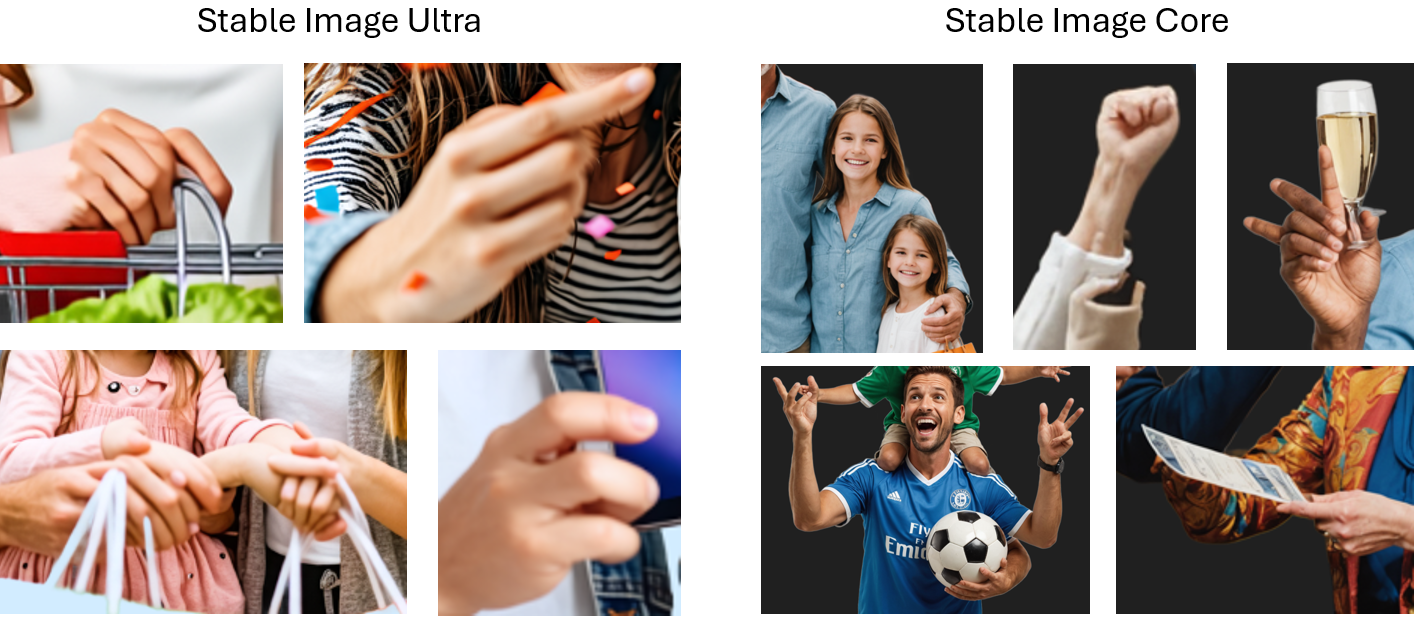
\includegraphics[width=1\linewidth]{Figures/erroresManos.png}
    \caption{Ejemplos de errores al graficar manos.}
    \label{fig:erroresManos}
\end{figure}

Otro tipo de error que se ha observado sobre todo en Stable Image Core es el de crear rostros distorsionados, con los ojos sin definir o viendo en dos direcciones diferentes. Además, este modelo tiende a colocar bigotes incluso en mujeres. Este tipo de errores se disminuyen al utilizar Stable Image Ultra. En la figura~\ref{fig:erroresManos} se pueden ver algunos ejemplos.

\begin{figure}[H]
    \centering
    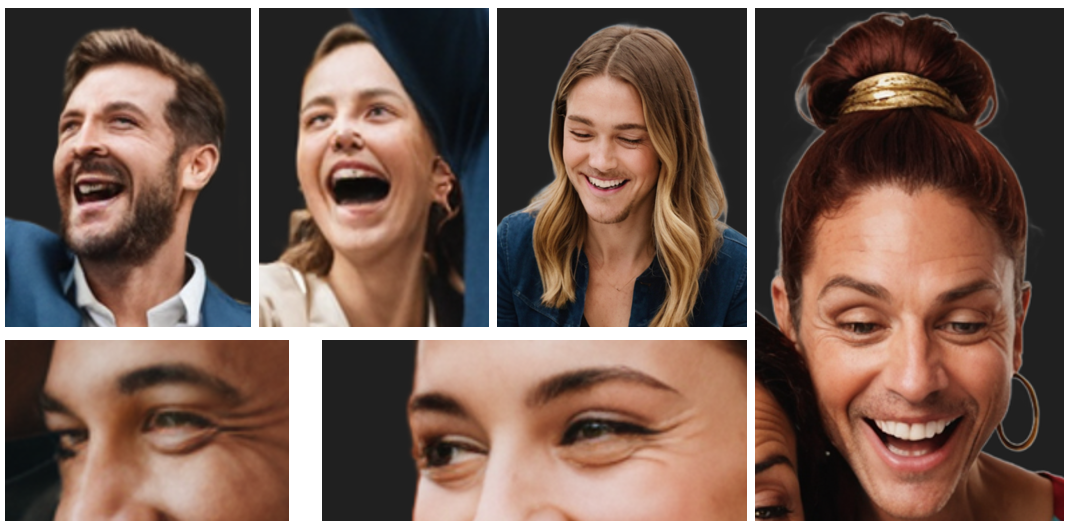
\includegraphics[width=1\linewidth]{Figures/erroresRostros.png}
    \caption{Ejemplos de errores al graficar rostros.}
    \label{fig:erroresManos}
\end{figure}

Por último, existen ocasiones en que, al remover el fondo, se quitan elementos que no correspondía eliminar. Esto ha pasado con mayor frecuencia al utilizar el servicio Stable Image Ultra, pero es un error que corresponde más a la herramienta de edición de imágenes. En la figura~\ref{fig:erroresFondo} se muestran ejemplos de este error.

\begin{figure}[H]
    \centering
    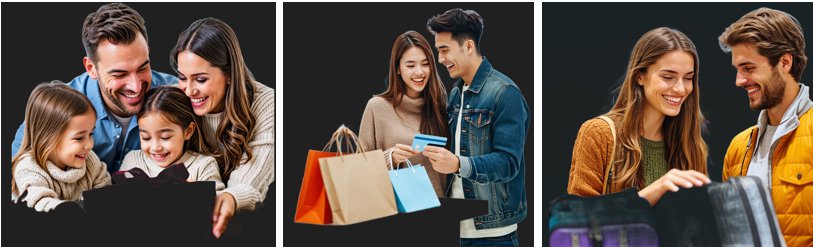
\includegraphics[width=1\linewidth]{Figures/erroresFondo.png}
    \caption{Ejemplos de errores de remoción de fondo.}
    \label{fig:erroresFondo}
\end{figure}

Una alternativa es evitar este paso al colocar la imagen completa como fondo de cabecera. Para lograrlo, se tendrían que realizar algunos pasos adicionales luego de generar la imagen. El primero sería hacer un escalado de la imagen para volverla más ancha de un lado. Luego se tendría que recortar para lograr el tamaño exacto de la cabecera. Finalmente, se debería imprimir el título del email sobre la imagen. 

Para clarificar, se puede observar un ejemplo en la figura~\ref{fig:cabeceraAlternativa}. Este tipo de diseño de cabecera ya es utilizado por la empresa y sería una alternativa interesante que quedaría pendiente por explorar.

\begin{figure}[H]
    \centering
    
\includegraphics[width=0.8\linewidth]{Figures/cabeceraAlternativa.png}
    \caption{Ejemplo de cabecera con imagen de fondo y título impreso encima.}
    \label{fig:cabeceraAlternativa}
\end{figure}

Luego de analizar los resultados queda pendiente resolver qué servicio es mejor utilizar, si Stable Image Core o su versión Ultra. Es difícil afirmar que el mayor precio del Ultra se compensa con sus mejores resultados ya que, como se mencionó anteriormente, su precio es 2,6 veces superior al servicio Core pero su aumento de efectividad no es el doble. Es cierto que al omitir el paso de la remoción del fondo, este modelo obtiene mejores resultados. Sin embargo, se puede concluir que conviene seguir generando alternativas de imágenes con ambos modelos para tener mayor variedad entre las cuales elegir.
